\subsection{Jednocestný usměrňovač}
\begin{figure}[h!]
    \centering
    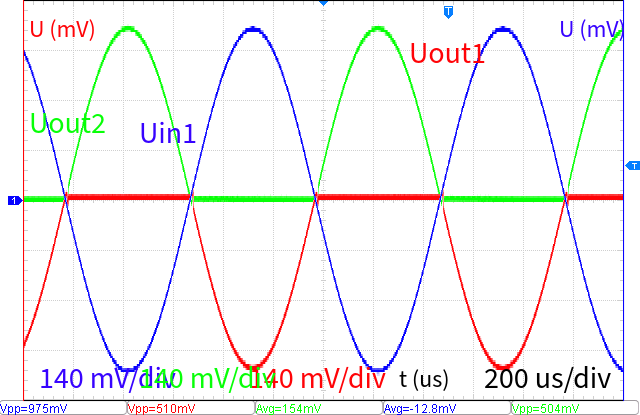
\includegraphics[width=0.56\textwidth]{lab/output1.png}
    \caption{Zapojení a) -- časová závislost obou výstupních signálů a vstupního signálu (f = \qty{1}{\kilo\hertz}, \(U_M\) = \qty{500}{\milli\volt})}
    \label{fig:lab/output1.png}
\end{figure}

\begin{figure}[h!]
    \centering
    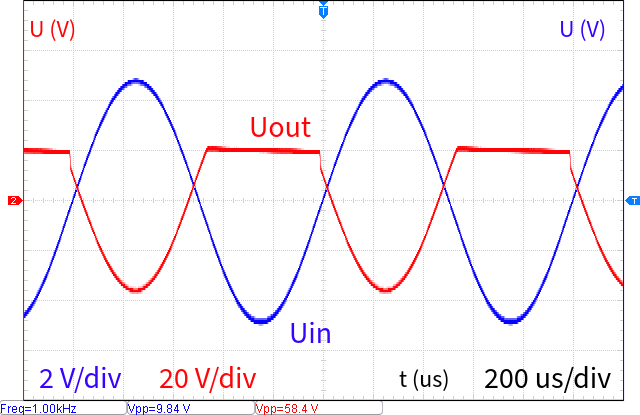
\includegraphics[width=0.56\textwidth]{lab/output3.png}
    \caption{Zapojení a) -- časová závislost stejných signálů, nejmenší dosažená amplituda, \(U_{M - min }=\qty{15}{mV}\).}
    \label{fig:lab-output3-png}
\end{figure}


\begin{figure}[h!]
    \centering
    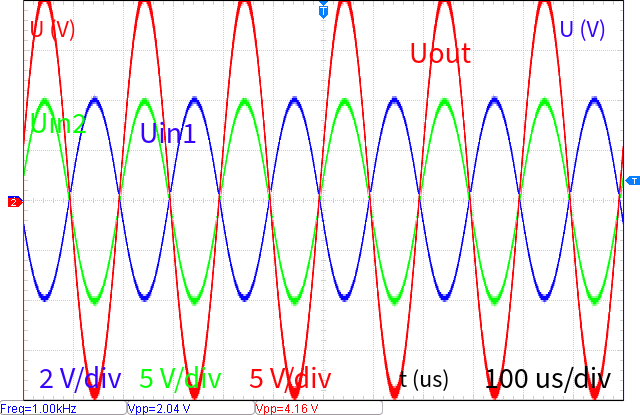
\includegraphics[width=0.56\textwidth]{lab/output5.png}
    \caption{Zapojení a) -- časová závislost vstupních a výstupních signálů při vyyšší frekvenci (\(f=\qty{5}{\kilo\hertz}\)), již jsou patrné drobné překmity.}
    \label{fig:lab-output5-png}
\end{figure}

\begin{figure}[h!]
    \centering
    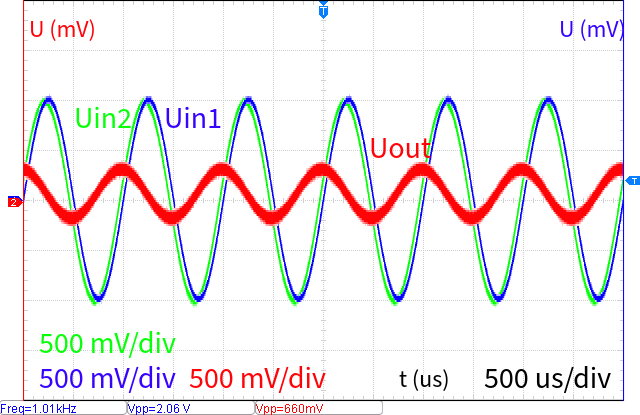
\includegraphics[width=0.56\textwidth]{lab/output6.png}
    \caption{Zapojení a) -- časová závislost vstupních a výstupních signálů při vysoké frekvenci (\(f=\qty{30}{\kilo\hertz}\)), jsou patrné výrazné překmity.}
    \label{fig:lab-output6-png}
\end{figure}

\clearpage
\subsection{Dvoucestný usměrňovač, zapojení b)}
\begin{figure}[h!]
    \centering
    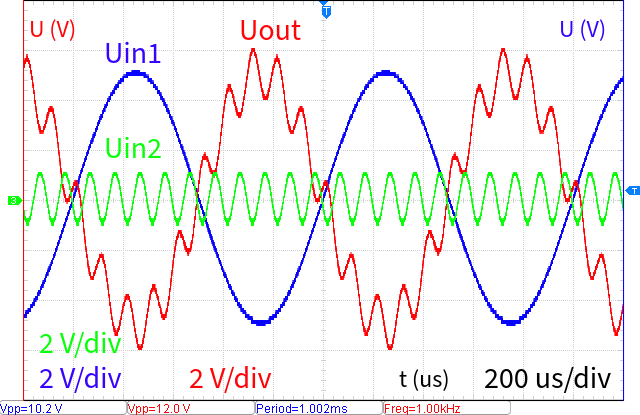
\includegraphics[width=0.56\textwidth]{lab/output7.png}
    \caption{Zapojení b) -- časová závislost signálů na vstupu, výstupu prvního OZ a celkovém výstupu zapojení, \(f=\qty{1}{\kilo\hertz}, U_M=\qty{1}{\volt}\).}
    \label{fig:lab-output7-png}
\end{figure}

\begin{figure}[h!]
    \centering
    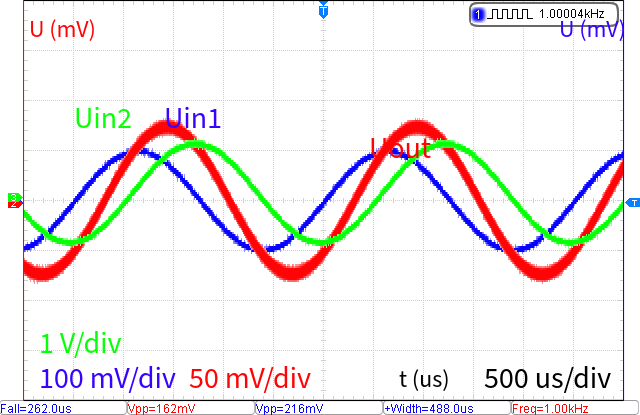
\includegraphics[width=0.56\textwidth]{lab/output8.png}
    \caption{Zapojení b) -- časová závislost stejných signálů, vyšší prekvence signálu (\(f=\qty{3}{\kilo\hertz}\)), překmity jsou patrné.}
    \label{fig:lab-output8-png}
\end{figure}

\begin{figure}[h!]
    \centering
    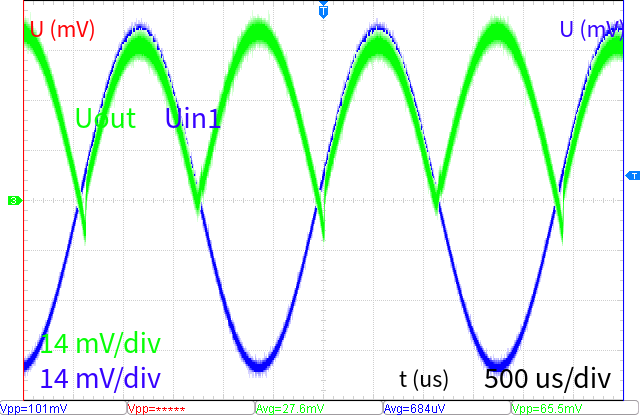
\includegraphics[width=0.56\textwidth]{lab/output9.png}
    \caption{Zapojení b) -- časová závislost vstupního a výstupního signálu, nejmenší dosažená amplituda, \(U_M=\qty{50}{\milli\volt}, f=\qty{419}{Hz}\)}
    \label{fig:lab-output9-png}
\end{figure}

\clearpage
\subsection{Dvoucestný usměrňovač, zapojení c)}
\begin{figure}[h!]
    \centering
    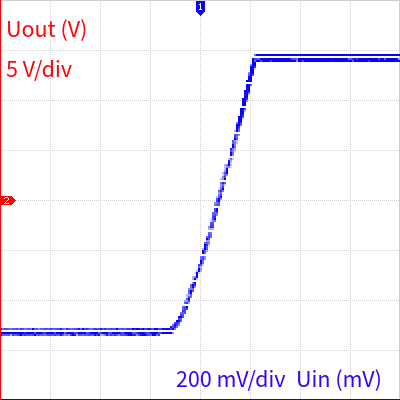
\includegraphics[width=0.56\textwidth]{lab/output10.png}
    \caption{Zapojení c) --  časová závislost signálů na vstupu, výstupu prvního OZ a celkovém výstupu zapojení, \(f=\qty{1}{\kilo\hertz}, U_M=\qty{500}{\milli\volt}\).}
    \label{fig:lab-output10-png}
\end{figure}

\begin{figure}[h!]
    \centering
    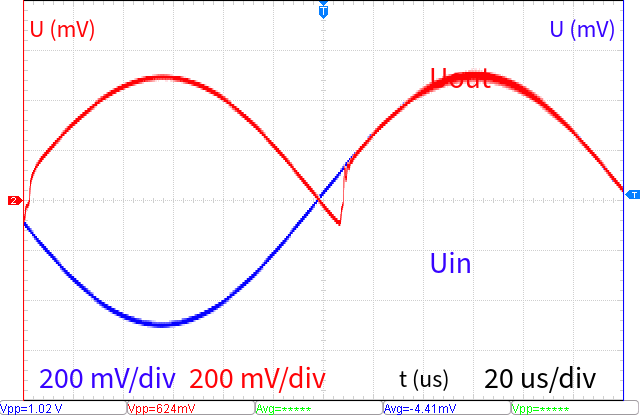
\includegraphics[width=0.56\textwidth]{lab/output11.png}
    \caption{Zapojení c) --  časová závislost signálů na vstupu a výstupu při vyšší frekvenci signálu (\(f=\qty{4}{\kilo\hertz}\)), již jsou patrné překmity.}
    \label{fig:lab-output11-png}
\end{figure}

\begin{figure}[h!]
    \centering
    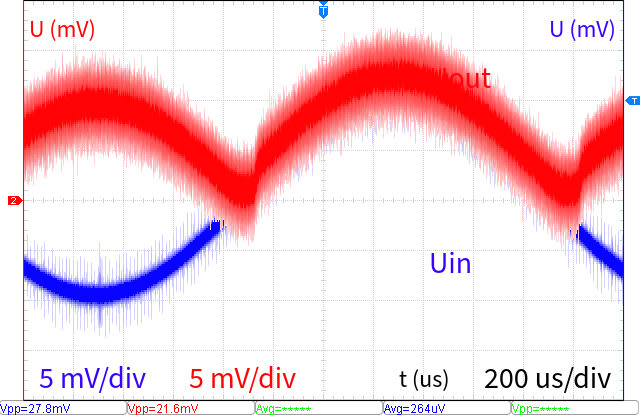
\includegraphics[width=0.56\textwidth]{lab/output12.png}
    \caption{Zapojení c) -- časová závislost signálu na vstupu a výstupu, nejnižší dosažená amplituda, \(f=\qty{420}{\hertz}, U_M=\qty{10}{\milli\volt}\).}
    \label{fig:lab-output12-png}
\end{figure}



\begin{table}[h!]
    \centering
    \def\arraystretch{1.4}
    \caption{Porovnání rozsahů, ve kterých zapojení usměrňují.}
    \begin{tabular}{|c|c|c|c|c|}
        \hline
            Zapojení & Sim.: \(U_{M-min} \)  & Měření: \(U_{M-min} \) & Sim.: \(f_{max} \) & Měření: \(f_{max} \) \\
        \hline
            a) & \qty{200}{\milli\volt} & \qty{15}{\milli\volt} & \qty{30}{\kilo\hertz} & \qty{5}{\kilo\hertz} \\
            b) & \qty{50}{\milli\volt} & \qty{50}{\milli\volt} & \qty{10}{\kilo\hertz} & \qty{3}{\kilo\hertz} \\
            c) & \qty{5}{\milli\volt} & \qty{10}{\milli\volt} & \qty{30}{\kilo\hertz} & \qty{4}{\kilo\hertz} \\
        \hline
    \end{tabular}
    \label{tab:dc-bod}
\end{table}